\chapter{Contexte du projet}
%\markboth{Chapitre 1 }{Contexte du projet} %pour afficher l'entete
%\addcontentsline{toc}{chapter}{Chapitre 1 : Contexte du projet}

\section{Introduction}
Le premier chapitre de ce rapport présente l'organisme d'accueil ainsi que notre projet.

Nous commençons par présenter l'entreprise, ses activités, et ses objectifs en matière de technologies connectées.

Ensuite, nous expliquons le contexte dans lequel s'inscrit ce projet, en évoquant les enjeux et les problématiques auxquels il répond.

Par la suite, nous exposons la méthodologie de travail que nous avons choisie et expliquons les raisons de ce choix.

Nous détaillons également les différents outils et technologies que nous utilisons au sein de notre projet.

Enfin, nous expliquons  les choix techniques que nous avons effectués pour répondre aux exigences de l'entreprise et assurer une infrastructure robuste et sécurisée.



\section{Présentation de l'organisme d'accueil }

Dans cette section, nous abordons la présentation de l'organisme d'accueil Zeta Engineering ainsi que son domaine d'activité.

\subsection{Organisme d'accueil}

Notre stage de projet de Mémoire de Mastère a été réalisé chez Zeta Engineering, un bureau d'étude multifonction appartenant au groupe Agexis \cite{agexis}, qui intervient sur la zone européenne et africaine. 

Le groupe Agexis est un bureau d'étude technique pluridisciplinaire et maître d'œuvre du bâtiment et des infrastructures. Il est implanté en Île-de-France depuis 2015. 

Zeta Engineering est spécialisée dans le consulting et l'ingénierie, et se consacre principalement aux conseils en communication, marketing, IT et gestion pour ses partenaires, en Tunisie comme en France. Elle est basée en Tunisie depuis 2018.

\subsection{Domaines d'activités}
Zeta Engineering, en collaboration avec Agexis et les autres membres du groupe, est chargée de mettre en place leur stratégie marketing pour la période 2020-2030, en déployant leur communication et leur commercialisation.

Cette entreprise de bureau d'études multifonctions est située en Tunisie et travaille en étroite collaboration avec Agexis. Les services proposés par Zeta Engineering sont très diversifiés et couvrent différents secteurs.
\section{Présentation du projet}

Dans cette section, nous abordons le cadre de notre projet, ainsi que la problématique de notre projet.

\subsection{Cadre de projet}
Dans le cadre de notre projet de Mémoire de Mastère, nous avons été accueillis au sein de Zeta Engineering. 

Notre mission consiste à mettre en place une infrastructure IT et SI pour relier les trois nouveau locaux \ref{tab1} de l'entreprise via un réseau MAN.\\


\begin{table}[H]
\begin{center}
     \begin{tabular}{|c{5cm}|c{5cm}|c{5cm}|}
    \hline
	\textbf{Logo}         & \textbf{Adresse}   & \textbf{Fonctionnalité} \\
    \hline
    
	
\includegraphics[width=4cm]{Images/logo-zeta1.png} & Rades Meliane, Rue de la Solidarité  & Réservé à l'administration et l'équipe diffusion globale  \\
	
 	\hline
 	
	\includegraphics[width=4cm]{Images/logo-Sequencia.png}   &  Rades, Rue Habib Bourgiba  &  Centre d'appel \\
	
	\hline
	
	
\includegraphics[width=4cm]{Images/Logo-ZetaProject.png}  & Ezzahra, Rue Habib Bourgiba    & Abrite les ingénieurs et les développeurs informatique  \\
	
	\hline
	
     \end{tabular}
     \caption{Les nouveaux locaux de Zeta Engineering en Tunisie}
     \label{1}
     \end{center}
     \label{tab1}
\end{table}

De suite, nous allons connecter les objets de l'entreprise tels que les machines de pointage, le capteur de température et humidité, les lampes, les smartphones et les caméras de surveillance dans notre système d'information pour une utilisation plus efficace de ces ressources au sein de l'entreprise.

\subsection{Problématique}
La problématique de notre projet s'articule autour de trois domaines distincts, chacun présentant ses propres défis.

Le premier défi réside dans l'isolation des trois bureaux de ZETA, les empêchant de former un réseau local (LAN). Cette absence de connectivité entre les bureaux pose un obstacle majeur à la communication et au partage d'informations entre eux.

Deuxièmement, nous nous sommes confrontés à un problème lié à la gestion des informations. Il manque un système d'information. Cela engendre des difficultés pour stocker, gérer et accéder aux données collectées par les divers applications.

Enfin, l'intégration des dispositifs IoT constitue une autre problématique majeure. La plupart de ces appareils ne disposent pas d'une connectivité native pour rejoindre notre réseau ni pour interagir avec le système d'information que nous prévoyons de mettre en place.

Nous nous attacherons à résoudre ces problématiques tout au long de notre projet, en développant des solutions adaptées à chaque domaine, visant à améliorer la connectivité entre les bureaux, à établir un système d'information efficace, et à faciliter l'intégration des dispositifs IoT dans notre infrastructure.

\section{Méthodologie de travail et planification}

Dans cette section, nous abordons la présentation d'une méthodologie, ainsi que la problématique de notre projet.


\subsection{Présentation de la méthodologie en cascade}

Parmi les diverses méthodologies de gestion de projets telles que le modèle en V, les méthodologies itératives, Scrum, et bien d'autres, nous avons choisi d'adopter le modèle en cascade pour notre projet. Également connue sous le nom de méthodologie séquentielle, cette approche est souvent préférée dans les projets de Mémoire de Mastère en raison de sa simplicité et de sa facilité de compréhension.

Dans cette méthodologie, chaque étape doit être achevée avant que la suivante puisse commencer. Les étapes ne peuvent pas être rétrogradées et doivent être exécutées dans l'ordre établi. Cela signifie que le projet doit être entièrement défini et spécifié avant que la conception ne puisse commencer, et que la conception doit être terminée avant que la mise en œuvre puisse commencer, et ainsi de suite.


La figure \ref{Chap1.4} illustre les étapes caractéristiques de la méthodologie en cascade. Cette approche linéaire  et séquentielle guide le projet à travers une série d'étapes bien définies.


\begin{figure}[H]
 \centering
    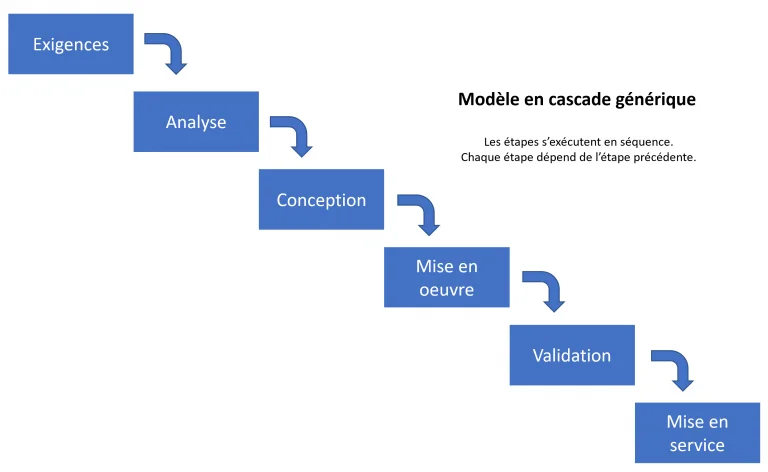
\includegraphics[width=15cm]{Images/cascade1.png}
    \caption{Méthodologie en Cascade \cite{blogcascade}}
    \label{Chap1.4}
\end{figure}

Le processus de la méthodologie en cascade se divise en plusieurs phases séquentielles, chacune étant une étape préalable à la suivante. Les étapes typiques incluent la définition des besoins, l'analyse, la conception, la mise en œuvre, les tests et la maintenance.



\subsection{Choix de la méthodologie en cascade}

Comme les besoins et les exigences du projet étaient relativement bien définis et stables dès le départ, le choix de la méthodologie en cascade s'est avéré approprié. Cette approche convient parfaitement lorsque les étapes du projet peuvent être planifiées à l'avance et que les changements ne sont pas fréquents.


De plus, notre équipe avait une compréhension claire des objectifs à atteindre et de la séquence des tâches à accomplir. La méthodologie en cascade nous a fourni un cadre structuré pour aborder chaque étape de manière méthodique, ce qui a permis une planification précise et une gestion efficace des ressources.



En résumé, chaque chapitre de notre rapport explique les choix matériels et logiciels adoptés, ainsi que la mise en œuvre de chaque composant du projet. Cette méthodologie nous permet de travailler de manière organisée et structurée, en veillant à ce que chaque étape soit achevée de manière adéquate avant de passer à la suivante \cite{fagarasan2021agile}.



\section{Outils et technologies utilisés}

Dans cette partie, nous allons détailler les différents outils et technologies que nous avons utilisés au sein de notre projet.

Cette présentation détaillée nous permettra de mieux comprendre les choix que nous avons effectués pour répondre aux exigences de l'entreprise et assurer une mise en œuvre réussie de notre projet.

\subsection{Matériels utilisés}

Dans cette sous-section, nous présentons le matériel utilisé pour la première partie Infrastructure IT, notamment les commutateurs, le pare-feu et les serveurs, sous forme d'un tableau \ref{1}.


\begin{table}[H]
\begin{center}
\begin{tabular}{|c{3cm}|c{3cm}|l{10cm}|}
\hline
\textbf{Image de l'équipement}         & \textbf{Nom de l'équipement}   & \textbf{Fonctionnalité} \\
\hline
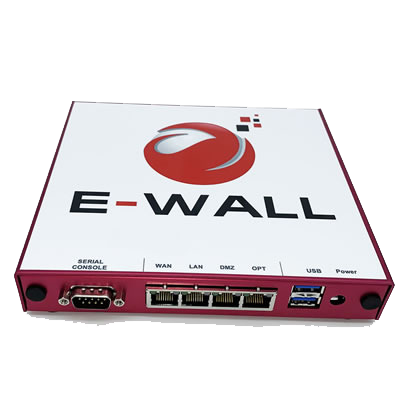
\includegraphics[width=3cm]{Images/ewall.png} & E-Wall Pare-Feu & E-Wall est une solution de sécurité essentielle pour protéger les réseaux informatiques contre les menaces externes. 

Son utilisation permet de renforcer la sécurité, de contrôler le trafic réseau et de détecter les activités malveillantes, contribuant ainsi à la préservation de l'intégrité, de la confidentialité et de la disponibilité des données. \\
\hline
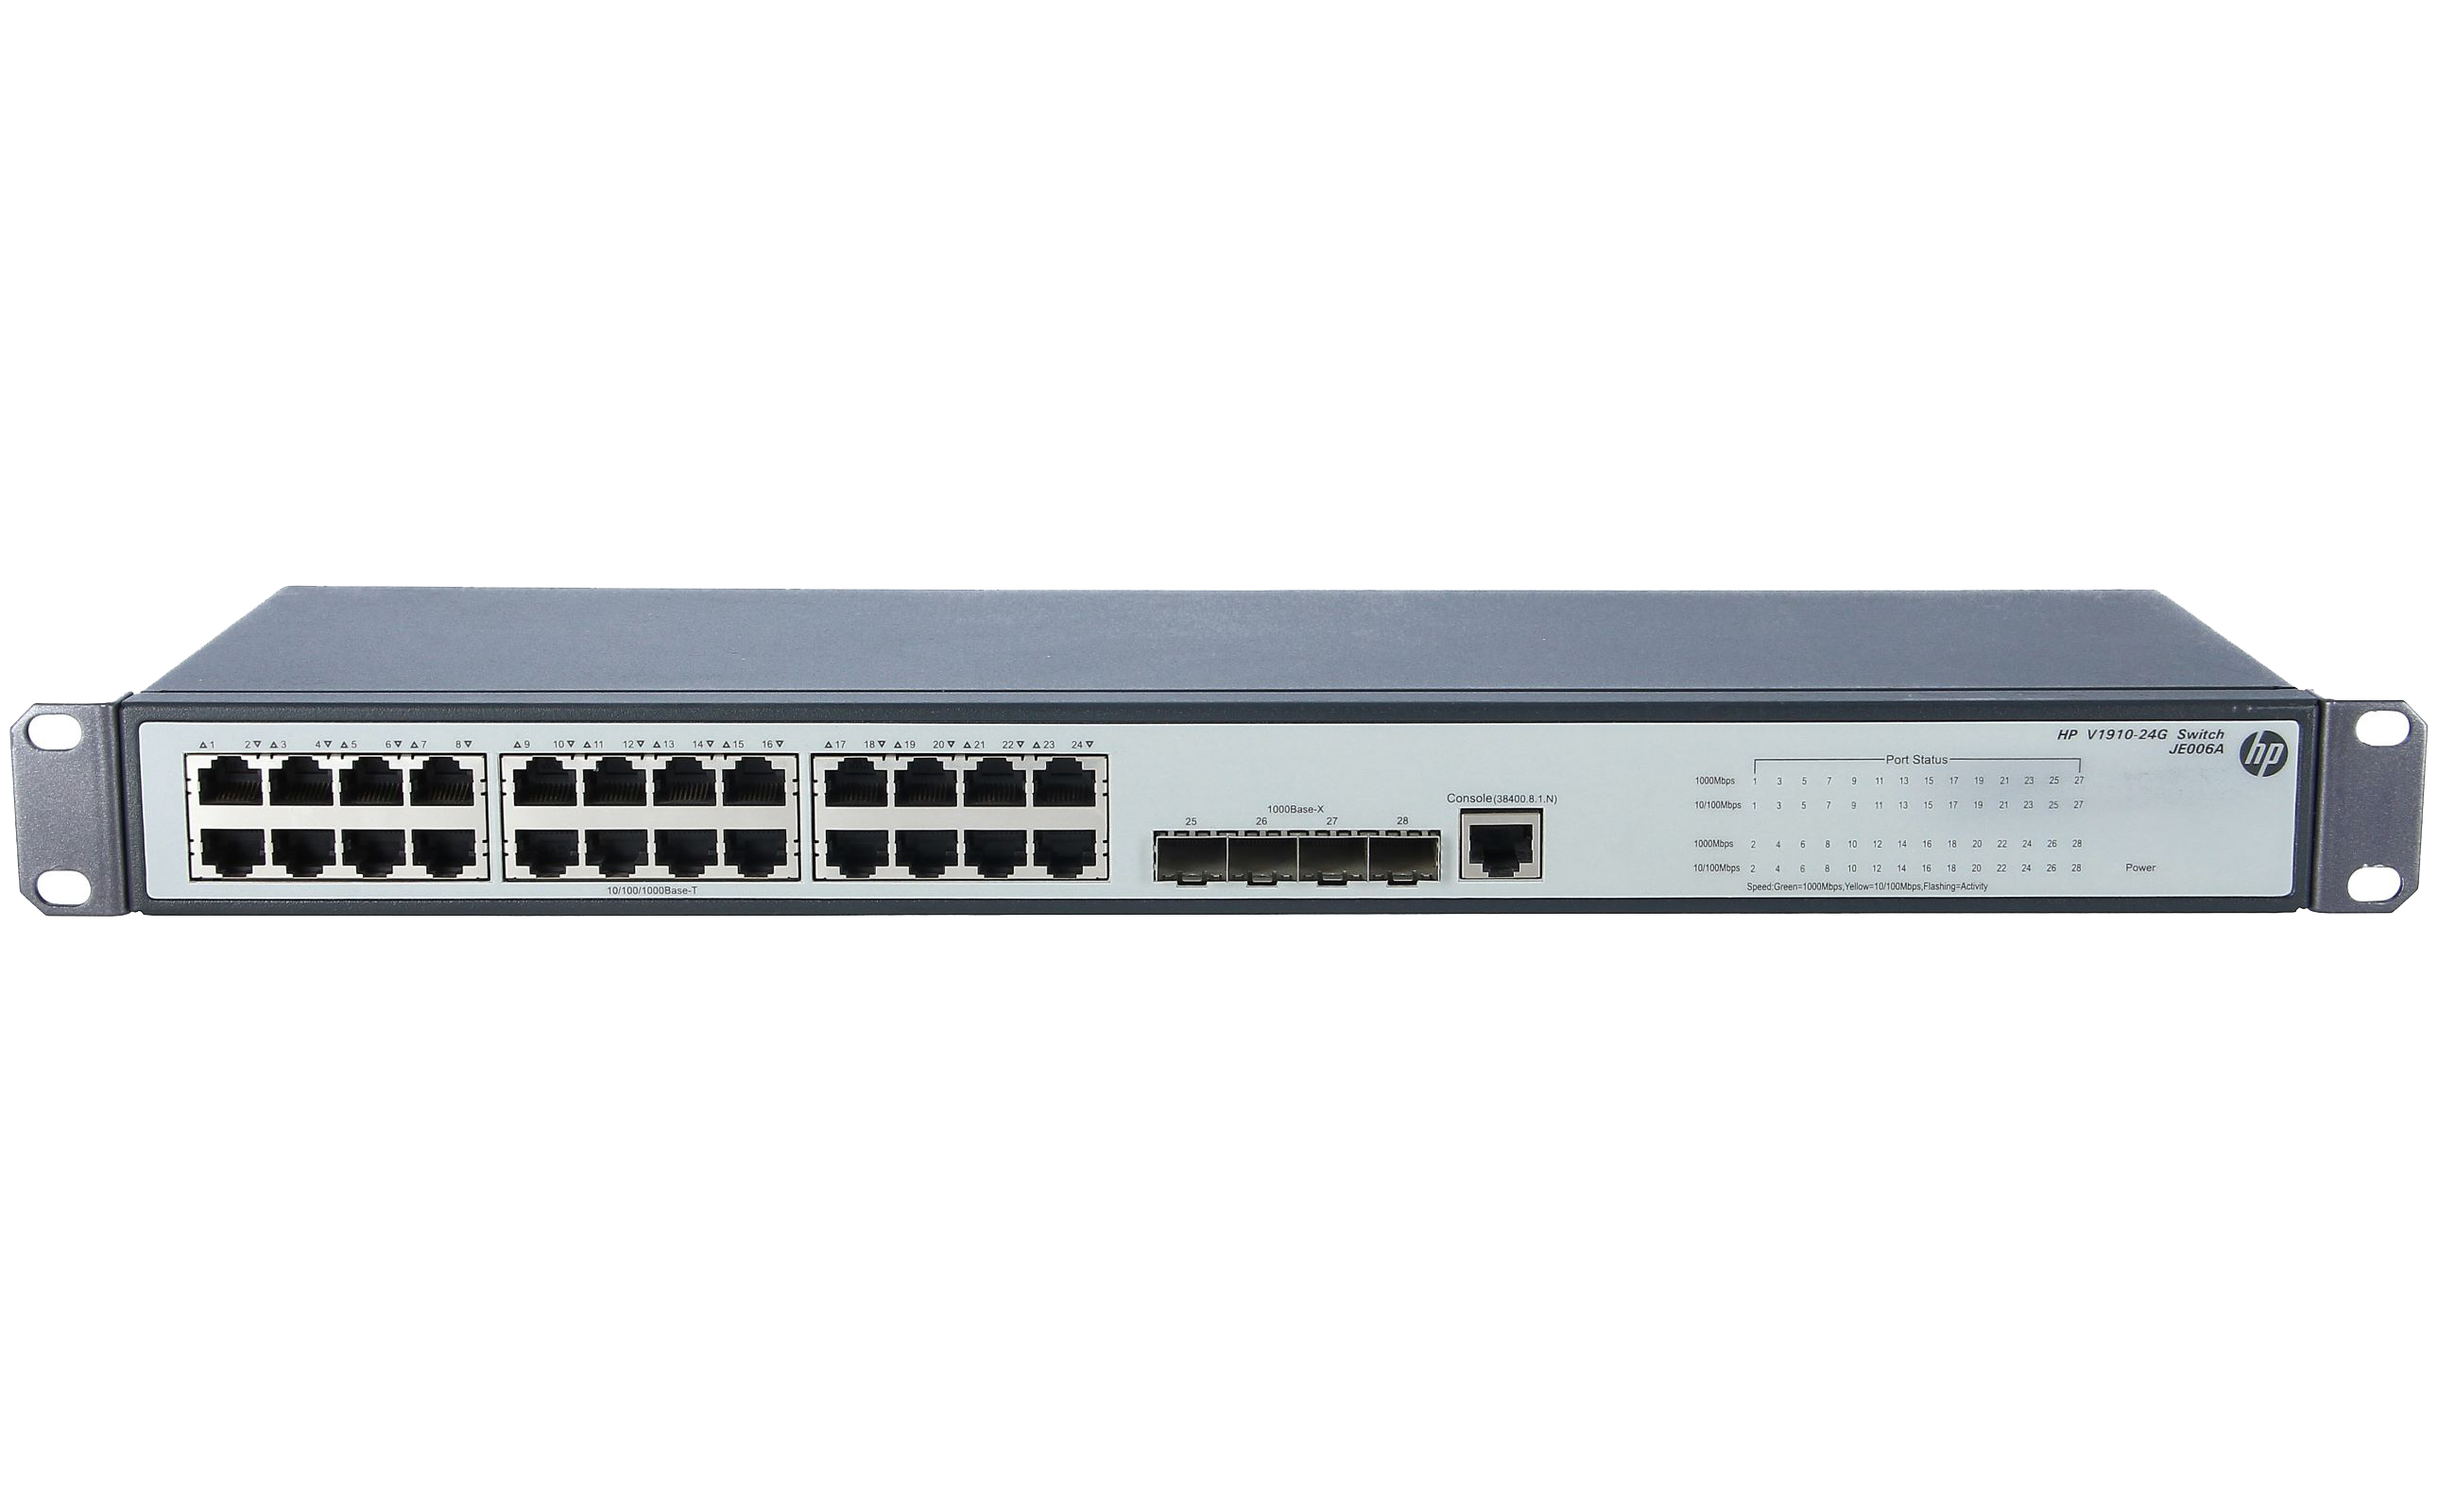
\includegraphics[width=3cm]{Images/HP1910.png} & Commutateurs HP1910 G24 & C'est un modèle de commutateur d'entreprise qui offre des fonctionnalités de gestion avancées pour les réseaux LAN. Il dispose de 24 ports Gigabit Ethernet et peut être géré via une interface web ou en ligne de commande. 

Il prend en charge les protocoles de gestion de réseau SNMP, RMON et LLDP, ainsi que les VLAN, le QoS, le STP et d'autres fonctionnalités de sécurité.  \\
\hline
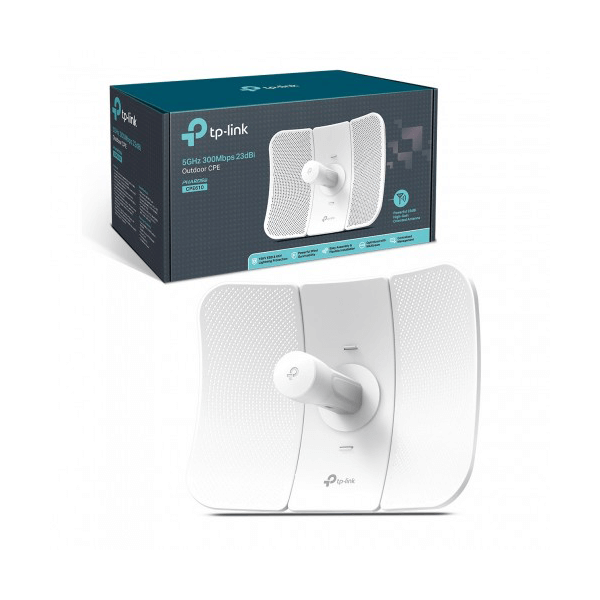
\includegraphics[width=3cm]{Images/TP-Link-CPE610-5GHz_1.png} & TP-Link CPE610 & Le TP-Link CPE610 est un point d'accès extérieur sans fil conçu pour fournir une connectivité Wi-Fi à longue portée dans des environnements extérieurs. 

Il utilise une antenne directionnelle à haut gain pour offrir des connexions sans fil stables et fiables sur de longues distances.  \\
\hline
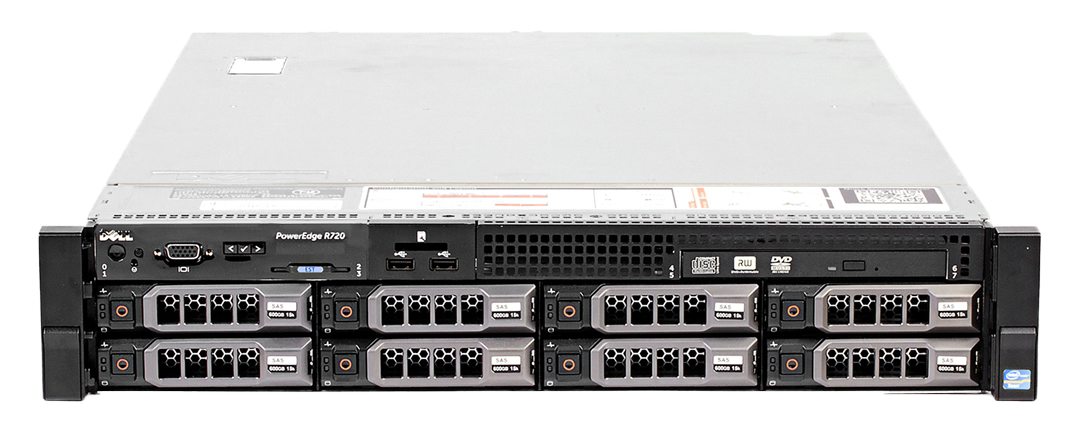
\includegraphics[width=3cm]{Images/dellr720.png} & Dell PowerEdge R720 & Le Dell PowerEdge R720 est un serveur rackable de haute performance, fiable et évolutif, offrant une grande capacité de stockage et de traitement de données pour les applications critiques de l'entreprise. 

Il est équipé de processeurs Intel Xeon E5-2600 v2 et peut prendre en charge jusqu'à 1,5 To de mémoire vive. Le PowerEdge R720 dispose également de fonctionnalités de haute disponibilité telles que les alimentations redondantes, les disques durs en miroir et les cartes réseau doubles. \\
\hline
\end{tabular}
\caption{Matériels utilisés}
\label{1}
\end{center}
\end{table}


\subsection{Logiciels utilisés}

Dans cette sous-section, nous présentons dans les tableaux \ref{2} et \ref{3} où sont répertoriés les logiciels utilisés tout au long de notre projet. 


\begin{table}[H]
\begin{tabular}{|c{3cm}|c{3cm}|l{10cm}|}
\hline
\textbf{Logo}         & \textbf{Nom de l'équipement}   & \textbf{Fonctionnalité} \\
\hline

\includegraphics[width=3cm]{Images/Logo-GNS3.png} & GNS3 & GNS3 est un logiciel open-source de simulation de réseaux informatiques. 

Il permet de créer des topologies réseau virtuelles en utilisant des images de routeurs, de commutateurs et d'autres équipements réseau. \\
\hline
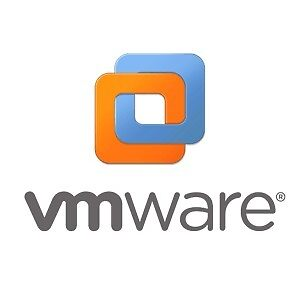
\includegraphics[width=3cm]{Images/Logo-VMWare.jpg}  & VMware Workstation & VMware Workstation est un logiciel de virtualisation puissant qui permet d'exécuter plusieurs systèmes d'exploitation sur une seule machine physique. 

Il offre la possibilité de créer et de gérer des machines virtuelles (VM) sur une plateforme hôte, ce qui permet d'exécuter plusieurs systèmes d'exploitation simultanément. VMware Workstation est disponible pour les principales plateformes telles que Windows, Linux et macOS. \\
\hline

\includegraphics[width=3cm]{Images/Logo-VNCViewer.png} & VNC Viewer & VNC Viewer est une application de bureau à distance qui permet de se connecter à un ordinateur distant et d'en contrôler l'écran et les applications à distance. 

Il offre la possibilité de se connecter à distance à des appareils tels que le Raspberry Pi, permettant ainsi une gestion et un contrôle pratiques de l'appareil à partir d'un autre ordinateur. \\
\hline

\includegraphics[width=3cm]{Images/Logo-IPScanner.png} & Advanced IP Scanner & Advanced IP Scanner est un outil de gestion de réseau qui permet de scanner rapidement un réseau et de trouver tous les périphériques connectés, y compris les ordinateurs, les imprimantes, les routeurs, les commutateurs, les caméras IP, etc.

Il permet également de détecter les adresses IP inactives et les ports ouverts sur les périphériques.  \\
\hline

\includegraphics[width=3cm]{Images/Logo-Fritzing.png} & Fritzing & Fritzing est un logiciel de conception électronique open-source qui permet de créer des schémas électroniques, des circuits imprimés et des modèles de connexion pour des projets électroniques. 

Il offre une interface conviviale et intuitive, ce qui facilite la création de schémas électroniques même pour les débutants. \\
\hline
\end{tabular}
\caption{Logiciels utilisés}
\label{2}
\end{table}


\begin{table}[H]
\begin{center}
\begin{tabular}{|c{3cm}|c{3cm}|l{10cm}|}
\hline
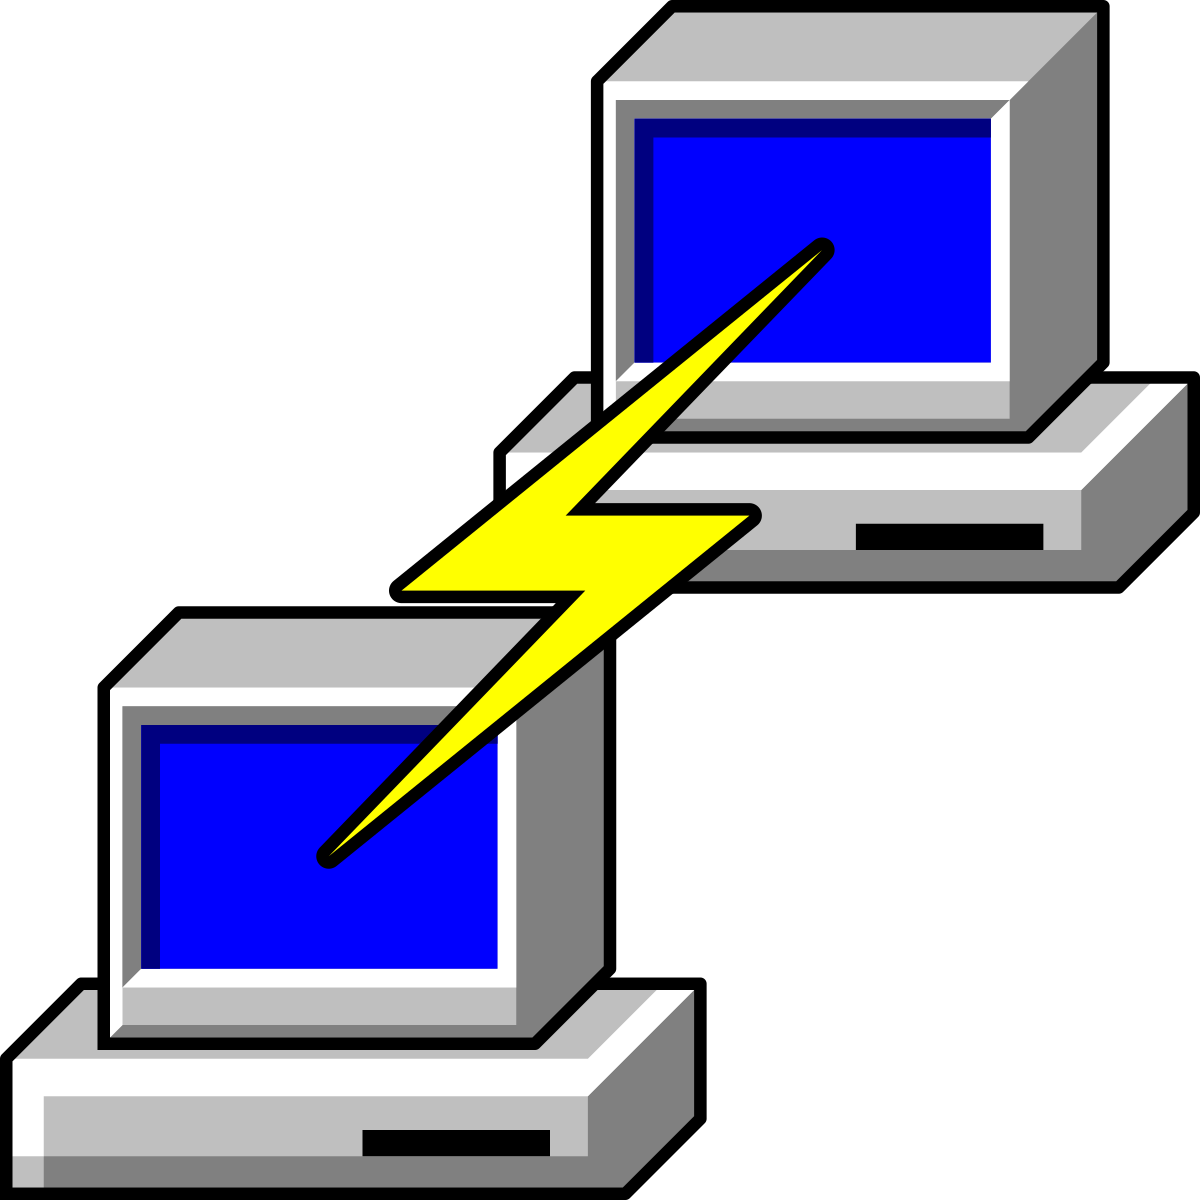
\includegraphics[width=3cm]{Images/Logo-Putty.png} & Putty & PuTTY est un logiciel client pour les protocoles de communication SSH, Telnet et Rlogin, permettant d'établir des connexions réseau sécurisées avec des ordinateurs distants. 

Il est utilisé principalement pour administrer des serveurs à distance, mais peut également être utilisé pour des transferts de fichiers et des sessions de console distantes. \\
\hline

\includegraphics[width=3cm]{Images/Logo-Raspberry.png} & Raspberry Pi Imager & Raspberry Pi Imager est un logiciel qui permet de facilement installer des systèmes d'exploitation sur une carte SD ou une clé USB pour Raspberry Pi. 

Il offre une interface graphique simple à utiliser pour sélectionner et télécharger les images d'OS disponibles. \\
\hline

\includegraphics[width=3cm]{Images/xminglogo.png} & Xming & Xming est un serveur d'affichage X open source qui permet d'exécuter des applications graphiques Linux sur des systèmes Windows. 

Il fournit un environnement graphique pour les applications Linux, ce qui permet aux utilisateurs de Windows d'accéder et d'interagir avec des applications Linux à distance. \\
\hline
\end{tabular}
\caption{Logiciels utilisés - Suite}
\label{3}
\end{center}
\end{table}




\section{Conclusion }
En conclusion, ce premier chapitre nous a permis de présenter l'organisme d'accueil, Zeta Engineering, ainsi que le contexte du projet consistant à ouvrir trois nouveaux bureaux à Rades, Rades Meliane et Ezzahra, et les défis qui en découlent.

Nous avons ensuite abordé la méthodologie choisie pour la gestion de ce projet, à savoir la méthode en cascade, qui nous permet de travailler de manière séquentielle en terminant chaque phase avant de passer à la suivante.

Les choix en matière de matériels et logiciels pour chaque étape sont également détaillés dans ce chapitre suivants, garantissant ainsi une bonne exécution du projet.